\section{Introduction}
\label{sec:intro}

We propose an agent memory without a generative writer. Here, a writer is a language model that selects and rewrites past interactions for storage. Our approach retains the original history and retrieves relevant evidence when a question arrives. Agent memories make information from earlier interactions available to later tasks \citep{packer2023memgpt,park2023generative}. Many use a generative model to construct the stored representation. Mem0 extracts and updates facts \citep{chhikara2025mem0}, Zep constructs a temporal knowledge graph \citep{rasmussen2025zep}, and Letta's agents edit memory files \citep{letta2025sleeptime,packer2023memgpt}. Workflow memories similarly use a model to derive guidance from past agent runs \citep{fang2026memp,ouyang2026reasoningbank,wang2025agent}.

Generative writing introduces three possible costs. First, extraction and update calls add ingestion cost as the history grows, even when no later question uses the stored information \citep{chhikara2025mem0,rasmussen2025zep}. Second, sampling can produce different stores from the same history, so reproducing a memory requires more than its construction code. Third, the writer can omit or alter details that later questions need. One audit of a Mem0 deployment classified 97.8 percent of 10,134 stored entries as junk \citep{mem0issue4573}; this is evidence from one deployment rather than a general failure rate. An agent that runs across thousands of sessions pays these costs on every one of them, while a benchmark score is paid for once, so we treat a memory result as a claim about accuracy together with tokens read, search time and build cost. We investigate what can be achieved without generative write calls. Our main LoCoMo comparison uses Mem0's published reader, judge and prompts on both sides.

Our memory stores each conversation turn verbatim, together with its speaker and date (Figure~\ref{fig:method}). To retrieve relevant evidence, we combine a keyword search for matching words with an embedding search for similarity in meaning. On LoCoMo, this produces an initial ranking of turns that we refine in three further stages. A dialogue rule passes part of each turn's score to the next turn in the same session, helping surface replies that do not repeat the question's words. A second rule boosts turns spoken by the person the question is about. Two local models, called cross-encoders, then rescore the leading candidates by evaluating each turn together with the question. A reader language model answers from the highest-ranked original turns, presented in chronological order. On LongMemEval-S, the keyword and embedding searches rank whole sessions without these later stages. We also adapt this retrieval approach to rank past agent trajectories on Proced-Mem \citep{procedmem}.

The answer comparison on LoCoMo has similar aggregate accuracy under a shared reader, judge and prompts from Mem0's published evaluation \citep{mem0benchmarks2026}. On the 607 questions both systems have answered, our store scores 90.6 against 90.3 while reading 3,294 tokens per question against 6,956, with no generative write calls. This aggregate includes 385 development questions used to tune the search. On the 222 test questions alone, our store scores 82.0 against 85.6. The full test split was not completed, so the aggregate result does not establish parity on unseen questions.

Retrieval can also be measured without a reader. Our store finds every gold session in the top 10 for 97.4 percent of 470 LongMemEval-S questions; EdgeMem and MemGAS report 93.8 and 94.5, respectively \citep{cui2026edgemem,xu2025memgas}. Our result includes scored questions from the 150-question development split used for tuning, and the comparison interprets the published retrieval metric as all-gold recall. On LoCoMo, the store retrieves 80.3 percent of gold turns in the top 10, against 64.0 for a flat fusion of the same two signals.

The error analysis identifies different weaknesses: model-written facts can lose detail on single-hop questions, while retrieval can omit a turn needed for a multi-hop answer. Two search changes motivated by these errors raise test all-gold recall from 90.2 to 94.4 at 150 turns. This measures the share of questions whose gold turns are all retrieved; no reader has been evaluated on the changed ranking. On Proced-Mem, the retriever reaches 0.957 mean average precision against the benchmark's 0.796. That retriever was selected on the same 40 queries used to score it.

Every main comparison in the paper is in Table~\ref{tab:headline} with its interval, and Figure~\ref{fig:beat} draws the main ones, so that a reader can see at once where the store beats, ties and loses. We mark the rows where tuning touched the scored questions, we state the judge on every row, and we claim a lead only where the difference lies outside its interval under a shared setup. Every run was registered with a prediction before it started, each miss is reported, and the runs that the model budget stopped are reported on the questions they finished and listed with their predictions in Section~\ref{sec:pending}.

Six terms recur. The reader is the language model that answers from the retrieved text, and the judge is the language model that marks an answer right or wrong. A gold turn is a turn the benchmark marks as evidence for the answer, and all-gold recall at $k$ is the share of questions whose gold turns are all among the top $k$ retrieved. A tuned mark (\tun{}) flags a row that includes questions the system was tuned on. A band is a comparison whose two sides were judged by different models; it places a system near another and does not rank them.

\begin{table*}[t]
\caption{Every main comparison in one place. Beats and loses mean the difference lies outside its 95\% interval or margin. Tie means it does not. Band means the two rows differ in judge and cannot be ranked. \tun{} marks a row that includes questions the system was tuned on. One judge means both systems' existing answers were re-scored by Claude Sonnet 5.5 under the same prompt. Section~\ref{sec:setup} gives the interval methods and the caveats on the published rows.}
\label{tab:headline}
\footnotesize
\centering
\setlength{\tabcolsep}{3.5pt}
\begin{tabular}{@{}L{40mm}rL{27mm}L{27mm}L{24mm}L{22mm}@{}}
\toprule
Benchmark and measure & Ours & Comparator & Difference & Setup & Verdict \\
\midrule
LongMemEval-S, all gold sessions in top 10, 470 q.\tun{} & 97.4 & EdgeMem 93.8 & +3.6, margin 2.6 & no reader; published metric inferred & beats \\
LongMemEval-S, all gold sessions in top 3, 470 q.\tun{} & 84.0 & EdgeMem 81.5 & +2.6, margin 4.8 & no reader; published metric inferred & tie \\
LoCoMo, share of gold turns in top 10, 1,152 test q. & 80.3 & flat fusion 64.0, our own baseline & +16.3 [+13.8, +19.2] & no reader & beats \\
Proced-Mem, MAP, 40 queries\tun{} & 0.957 & MiniLM baseline 0.796 & +0.16; judge moves a ranking by up to 0.08 & same judge; no held-out split & beats \\
LoCoMo single-hop accuracy, 256 shared q.\tun{} & 95.7 & Mem0 90.6 & +5.1 [+2.6, +9.2]; the 56 test q. alone +7.1 [$-$1.8, +16.1] & same reader, judge, prompts & beats; tie on test alone \\
LoCoMo accuracy, 607 shared q.\tun{}; tokens 3,294 vs 6,956 & 90.6 & Mem0 90.3 & +0.3 [$-$3.6, +3.6] & same reader, judge, prompts & tie \\
LoCoMo accuracy, the 222 test q. both answered & 82.0 & Mem0 85.6 & $-$3.6 [$-$7.1, $-$0.5] & same reader, judge, prompts & loses \\
LoCoMo accuracy, 607 shared q.\tun{}, one judge & 90.1 & Mem0 90.0 & +0.2 [$-$4.6, +3.5] & same reader and prompts; Claude Sonnet 5.5 judges both & tie \\
LoCoMo accuracy, the 222 test q., one judge & 80.6 & Mem0 85.6 & $-$5.0 [$-$8.1, $-$1.4] & same reader and prompts; Claude Sonnet 5.5 judges both & loses \\
LoCoMo multi-hop accuracy, 130 shared q.\tun{} & 88.5 & Mem0 94.6 & $-$6.2 [$-$11.3, $-$2.5] & same reader, judge, prompts & loses \\
LongMemEval-S accuracy, 319 test q.\tun{}; tokens 19,125 vs 6,787 & 94.0 & Mem0 93.4 on 500 & +0.6 & same reader & band \\
BEAM 1M pass rate, 652 q. & 71.8 & Mem0 70.1 on 700 & +1.7 & same reader & band \\
BEAM 1M pass rate, 652 q., one judge & 61.3 & Mem0 63.9 on 700 & $-$2.6; intervals [57.6, 65.0] and [60.2, 67.3] & same reader; Claude Sonnet 5.5 judges both & tie \\
LoCoMo search time per question, seconds & 1.05 & Mem0 current 3.57, hosted mean; Mem0 2025 paper 0.200, own hardware & $-$2.52 s; +0.85 s & our laptop median; no shared hardware & beats the hosted mean; loses to the 2025 row \\
LoCoMo accuracy, best published row, any reader\tun{} & 90.6 & Zep 94.7, gpt-5.4, third party & $-$4.1 & different reader and judge & band \\
LongMemEval-S accuracy, best published row, any reader & 94.0 & Mastra 94.9, gpt-5-mini & $-$0.9 & different reader and judge & band \\
\bottomrule
\end{tabular}
\end{table*}

\begin{figure*}[t]
\centering
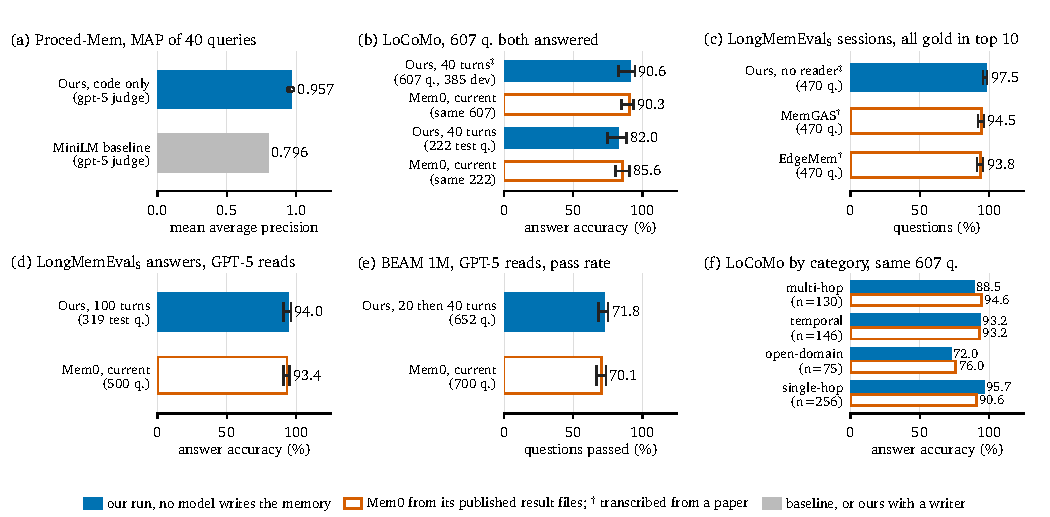
\includegraphics[width=\textwidth]{fig_beat.pdf}
\caption{The main comparisons. Filled bars are our runs. Hollow bars are other systems, read from their published per-question result files unless marked \pub{} (transcribed from a paper). Whiskers are 95\% intervals: conversation-cluster bootstrap in (b), Wilson score intervals for counts out of $n$ elsewhere. (b) and (f) use the 607 LoCoMo questions that both our GPT-5 run and Mem0's file have answered, with Mem0's answer and judge prompts and GPT-5 as reader and judge on both sides; 385 of the 607 are development questions on which the search weights were set (\tun{}), and the lower pair in (b) is the 222 test questions alone. (c) is retrieval with no reader, read as \rall{10}. (d) Our row uses the official LongMemEval judge; Mem0's row uses GPT-5 with its own judge prompt. (e) Our row uses BEAM's judge on gpt-4.1-mini; Mem0's uses GPT-5 with its own prompt. Dots in (a) are the three judge passes.}
\label{fig:beat}
\end{figure*}
